\documentclass[conference,11pt,letterpaper]{IEEEtran}

\usepackage[english]{babel}
\usepackage{csquotes}

\usepackage{fancyhdr}
\usepackage{extramarks}
\usepackage{mathtools}
\usepackage{amsthm}
\usepackage{amsfonts}
\usepackage{tikz}
\usepackage[plain]{algorithm}
\usepackage{setspace}
\usepackage{enumerate}
\usepackage{hyperref}
\usepackage{siunitx}
\usepackage{chngcntr}
\usepackage{graphicx}
\usetikzlibrary{automata,positioning}
\usepackage{wrapfig}
\usepackage{todonotes}
\usepackage{subcaption}
\usepackage{todonotes}
\usepackage{cleveref}
\usepackage{caption}

\captionsetup{font={footnotesize,it},labelfont={footnotesize,bf,it}}

\usepackage[style=authoryear,citestyle=authoryear-comp,maxcitenames=1,backend=biber,backref=false,doi=false,isbn=false,url=false,sorting=nyt]{biblatex}

\addbibresource{quadruped-gait-writeup.bib}

\renewcommand{\bibfont}{\footnotesize}
\setlength\bibitemsep{8pt}


\usepackage[no-math]{fontspec}
\setsansfont{DejaVu Sans}%{Arial}
\setmainfont{Linux Libertine O}%{Times New Roman}
\setmonofont{Inconsolata}%{Consolas}


\captionsetup{compatibility=false}

\emergencystretch=\maxdimen
\hyphenpenalty=10000
\hbadness=10000

\begin{document}
%
% paper title
% Titles are generally capitalized except for words such as a, an, and, as,
% at, but, by, for, in, nor, of, on, or, the, to and up, which are usually
% not capitalized unless they are the first or last word of the title.
% Linebreaks \\ can be used within to get better formatting as desired.
% Do not put math or special symbols in the title.
\title{\LARGE Studying Quadrupedal Gaits in Simulation\\\Large An Optimization-Inspired Approach}

% author names and affiliations
% use a multiple column layout for up to three different
% affiliations
\author{\IEEEauthorblockN{Alexander Volkov}
\IEEEauthorblockA{Robotics Institute\\
Carnegie Mellon University\\
5000 Forbes Ave., Pittsburgh, PA 15213\\
\texttt{avolkovjr@cmu.edu}}}

% make the title area
\maketitle

% As a general rule, do not put math, special symbols or citations
% in the abstract
\begin{abstract}

Of special interest in the study of legged locomotion is the variety of steady-state gaits exhibited by biological quadrupeds, as well as their preference for certain gaits based on locomotive efficiency and desired speed. In this work, I show that a similar collection of gaits and selection policy naturally emerges for a robotic quadruped. To this end, a high-fidelity dynamic model of the quadrupedal Ghost Robotics \emph{Minitaur} robot was developed and its emergent gait properties studied in simulation.
\end{abstract}

\section{Introduction}

% The introduction should introduce readers to the broader field within which your work is placed, and then guide them to the specific problem that you are addressing and why. Appropriately referencing the work of others to support claims made in the introduction is important here.

The variety of steady-state gaits exhibited by biological quadrupeds has long been of great interest in biomechanics. Previous work \autocite{hoyt_taylor_1981,hegland_taylor_1988} has associated such gait preference in a variety of wild and domestic animals with minimization of power expenditure, depending on desired speed. The ubiquity of this phenomenon in the biological domain motivates an effort to investigate whether a similar gait variety and selection policy naturally emerges on a robotic quadruped, despite the significantly different energy storage, transmission, and actuation mechanisms involved.

In this work, a high-fidelity dynamic model of a quadrupedal robot platform is used to generate and study the emergence of various steady-state gaits commonly observed in biological quadrupedal systems. A na{\"i}ve control architecture consisting of an elliptical foot trajectory generator, softly-tuned joint position PID controllers, and a low-dimensional gait timing parametrization (inspired by \autocite{Hildebrand701}) are used to emphasize the inherent, open-loop robustness of the system for valid gaits. 

Previous efforts on this project yielded promising initial results, but were largely impeded by the difficulty in achieving sufficient sampling granularity over the gait parameter space due to the brute-force evaluation approach taken and the nontrivial time required to compute each simulation trial. 

A more effective sampling method was desired, with the property that it would be biased toward greater sampling granularity near the sparsely distributed regions of interest corresponding to the quadruped's stable gaits. Recognizing that the evaluation of each sample provides an inherent performance metric (the gait efficiency, see \cref{sec:performance}) with local maxima corresponding to the regions of interest, the desired sampling method was reinterpreted as a form of optimization. However, rather than exclusively consider the terminal result of the optimization process, all intermediate steps of the search would be retained to construct a sampled approximation of the gait efficiency over the parameter space. Additional minor considerations would also be required to ensure that such an optimization algorithm is biased against early termination, in favor of searching more aggressively for alternative regions of interest in the parameter space.

The Covariance Matrix Adaptation Evolution Strategy (CMA-ES) optimization algorithm \autocite{hansen2001} was selected based on the foregoing considerations. A brief overview of the algorithm is provided in \cref{sec:cmaes}. A custom \emph{MATLAB} implementation of the CMA-ES algorithm was developed in order to make use of the computing environment's parallelization capabilities as well as interface directly with an existing \emph{Simulink/Simscape Multibody} physics simulation environment from previous work on this project. The resulting pipeline samples the gait parameter space far more efficiently than the previously used brute-force approach.

\subsection{Performance Evaluation} \label{sec:performance}

For the purposes of this study, gait performance was evaluated exclusively in terms of efficiency. Robustness to environmental disturbances was not of concern; a flat, high-friction ground model is used throughout the study. As is standard in locomotion literature \autocite{von1950price}, steady-state gait performance was quantified using the cost of transport (CoT) metric, as per \cref{eq:cot}:

    \begin{equation} \label{eq:cot}
        \text{CoT} = \frac{P_{in_{avg}}}{m_{sys}gv_{avg}} = \frac{E_{in_{tot}}}{m_{sys}gd_{tot}}
    \end{equation}
where $P_{in_{avg}}$ and $E_{in_{tot}}$ are the average power and total energy, respectively, provided to the system over a fixed time period in steady-state locomotion; $v_{avg}$ and $d_{tot}$ are the average velocity of and total distance travelled by, respectively, the system over the same interval; $m_{sys}$ is the total system mass; and $g$ is the acceleration due to gravity.

It should be noted that gait stability and efficiency are highly coupled. Infeasible or otherwise unstable gaits result in very high CoT evaluations, whereas stable gaits are comparably far more energetically effective.

\subsection{CMA-ES Algorithm} \label{sec:cmaes}

\todo{cmaes algorithm pseudocode + description}

\todo{review and edit everything below this}

\subsection{Minitaur Robot}

The simulated gait investigation reported here was done using a high-fidelity rigid-body model of a \emph{Ghost Robotics Minitaur} \autocite{grminitaur}: an 8 DOF, direct-drive (electrically actuated) quadrupedal robot platform capable of both quasi-static and dynamic gaits. A photo of the \emph{Minitaur} is provided in \cref{fig:grminitaur}.

\begin{figure}[ht!]
    \centering
    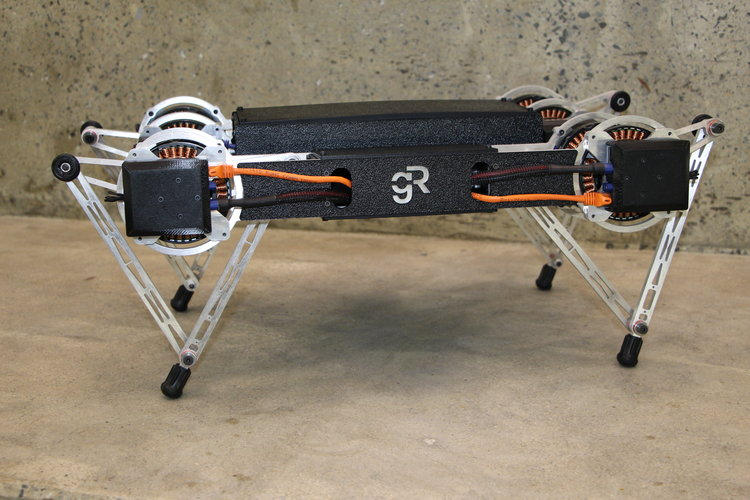
\includegraphics[width=0.48\textwidth]{grminitaur}
    \caption{Ghost Robotics Minitaur Platform \autocite{grminitaur}}
    \label{fig:grminitaur}
\end{figure}

\section{Model}


% TODO: Fix this transition based on how the intro ends\

Although spring-mass models such as SLIP and LIPM are popular for gait synthesis and control in contemporary legged robotics literature \autocite{albertwuhartmutgeyer2013}, their low-dimensional nature does not capture the complex dynamics that result with respect to both the variety of possible quadrupedal gaits as well as their relationship to the system's locomotive efficiency. Higher-dimensional lumped element models have also been studied as a means of simplifying and abstracting the mechanics of quadrupedal systems while nonetheless capturing their principle dynamic behaviors \autocite{remy2011optimal}. The construction of such reductive models inherently depends on a-priori knowledge of the systems' principle dynamics.

For our investigation, however, a high-fidelity model is needed in order to accurately capture the full system dynamics and power expenditure of the system. In effect, this maximally avoids introducing any simplifications that may inadvertently alter the emergent gait patterns and selection policies.

To this end, a detailed model of the \emph{Minitaur} was created in \emph{Simulink/Simscape Multibody}, with kinematic and inertial properties extracted directly from an accurate CAD model of the robot. The model includes a global trajectory generator for implementing different gaits; motor controllers to follow the generated trajectories; as well as motor, kinematic, and contact models for the \emph{Minitaur} platform. The description of each portion of the model follows.

\subsection{Trajectory Generator and Gait Parametrization}
For this project, we generate elliptical trajectories for each foot. An ellipse was chosen as it is simple enough to be easily parameterized, yet produces complex gait behavior. The major and minor diameters of the ellipse, its distance from the motor axes, and its tilt were determined manually by examining the reachable workspace of the foot as well as simulation to ensure stable behavior. The \emph{period} of the elliptical trajectory, which describes how long it takes for each foot to complete one pass through the ellipse, is given as a parameter to the system. To produce different gaits, a phase offset is given for each foot; that is, all feet follow the same trajectory with the same period, but at different phase offsets.  We represent the phase offsets using two parameters. The first is the \emph{left/right sync}, which is true if the left and right sides are symmetrical and false if they are antisymmetrical, (i.e., $180^\circ$ out of phase). The second parameter is the \emph{phase offset} of the fore legs, which determines how much each fore foot lags behind the corresponding back foot. From these parameters, we can generate a wide variety of gaits.


\subsection{Motor Controllers}
An analytical inverse kinematics model is used to compute desired motor angle from each foot trajectory. These desired joint angles are then fed into a softly-tuned position PID controller to compute desired motor torques, which are then sent to the motors. The "softness" of the position controller was used to emulation elasticity in the leg actuation. The gains were manually tuned to achieve acceptable performance. 

\subsection{Robot Model}
The \emph{Simulink/Simscape Multibody} model of the \emph{Minitaur}'s behavior includes several detailed features that make it more complicated than some of the simplified mechanical models we have discussed in class and make it more challenging to work with analytically. The mechanical model itself was generated from a CAD model supplied by Ghost Robotics and cleaned up manually by us. It includes details such as mechanical mates, material properties, and linkages. The motors are represented using a simplified brushless DC motor model, with a time constant delay in torque acquisition and saturation limits given by the motor specs. Joint friction is also modeled. For the ground contacts, a sphere-on-plane proportional-derivative model was used, sourced from a third-party Simscape contact model package \autocite{contactmodel}. This model contains both static and dynamic friction, and is sophisticated enough to demonstrate several gaits. Due to the complexity of the model itself, it is surprising that a simplified controller can produce complex gait behavior.

\section{Results}

To correlate the CoT with the parameters of the model, simulations were performed various values for the period of the gait and the phase offset between the fore leg and the hind leg, using CMA-ES with a large parameter space. Based on the results achieved, the parameter space for the period was narrowed down, and CMA-ES was conducted again.

\subsection{Parameter Sweep}
First, the entire parameter space was intelligently searched for \emph{period} $t \in[0.5,4]$ and the \emph{phase offset} $l \in[0,2\pi]$, with $0$ indicating in-phase and $\pi$ indicating out-of-phase motion of the fore and the hind legs using CMA-ES. This entire parameter space was searched for the two cases of left/right symmetry and anti-symmetry. The elliptical path trajectory for the simulation was a semi-major axis of radius $0.3\ell_{leg}$ oriented along the distance travelled and a semi-minor axis of radius $0.2\ell_{leg}$ length oriented vertically. 

\subsection{Preliminary Results}
The CoT heat map for left/right symmetric gaits can be seen in \cref{fig:sync_gait}. The majority of the parameters swept resulted in high CoT values. Local minima can be seen which correspond to bounding and pronking gaits. In the areas with large CoT, the \emph{Minitaur} simulation did not have enough energy input during the simulation and therefore was unable to move forward.
           \begin{figure}[ht!]
         
           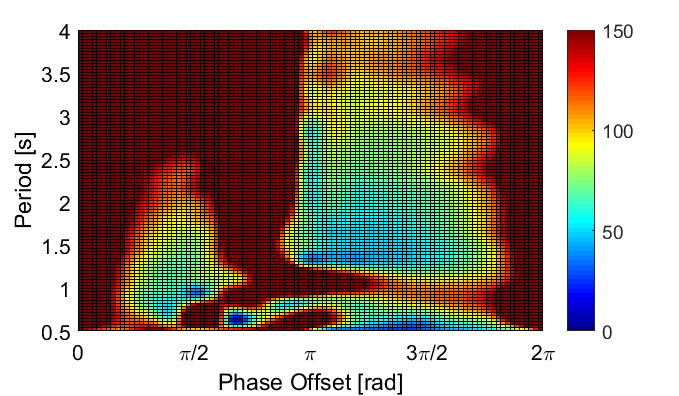
\includegraphics[width=0.53\textwidth]{smooth_CoT_sync_gait}
           \caption{CoT for left/right symmetric gaits}
           \label{fig:sync_gait}
           \end{figure}
                      \begin{figure}[ht!]
The CoT heat map for left/right anti-symmetric gaits similarly yielded local minima which corresponded with walking and trotting gaits (\cref{fig:unsync_gait}). In both heat maps, the minimum CoT occurred at very small periods, which is in accordance with biology where smaller animals tend to have gaits with higher frequencies.         
           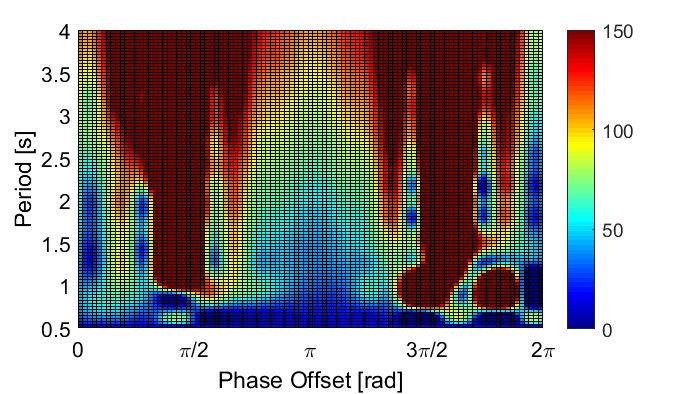
\includegraphics[width=0.53\textwidth]{smooth_CoT_unsync_gait}
           \caption{CoT for left/right anti-symmetric gaits}
           \label{fig:unsync_gait}
           \end{figure}
% TODO: THU can you fill in this section ?
% I am not sure what had you mentioned during the presentation 

\subsection{Refined Results}
Because the CoT minima occurred during smaller periods, the second simulation used a narrower period space, starting at 0.25s and ending at 1s. The period offset space was again 0 to 1. This entire parameter space was searched for symmetric and anti-symmetric gaits. The parameter space was narrowed in order to search more parameters in the space that produced lower CoT gaits.

The path trajectory for the simulation was changed because in the first experiment, the \emph{Minitaur} was unable to lift its legs off of the ground due to an inadequate path trajectory. Therefore, the elliptical path trajectory for the simulation was a semi-major axis with radius $0.5\ell_{leg}$ and a semi-minor axis of radius $0.3\ell_{leg}$, which are trotting trajectories for horses \autocite {mcmahon_1985}.

The minimum in CoT for left/right symmetric gaits was 34.6 occurring at a period of 0.58s and a phase offset of 1.1$\pi$ (\cref{fig:sync_gait_2}). The simulation was unstable in every phase offset condition at periods below 0.5s. In the left/right anti-symmetric gaits, the minimum CoT was 11.5 occurring at a period of 0.33s and a phase offset of 0.9$\pi $ (\cref{fig:unsync_gait_2}). The simulation had unstable gaits at every phase offset below 0.45$\pi$ and above 1.1$\pi$. 
\begin{figure}[ht!]
         
           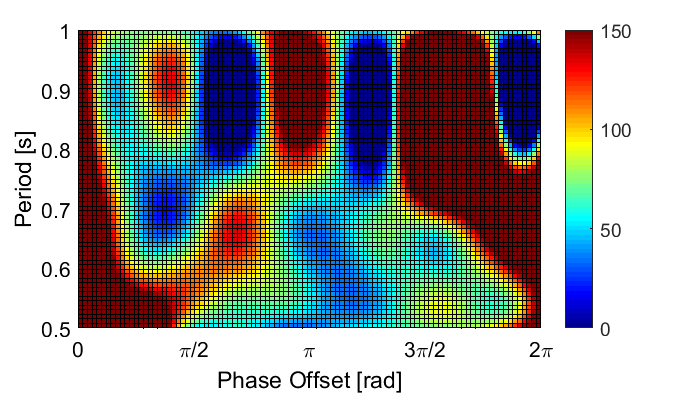
\includegraphics[width=0.53\textwidth]{sync}
           \caption{CoT for left/right symmetric gaits at smaller periods}
           \label{fig:sync_gait_2}
           \end{figure}
           
          \begin{figure}[ht!]
           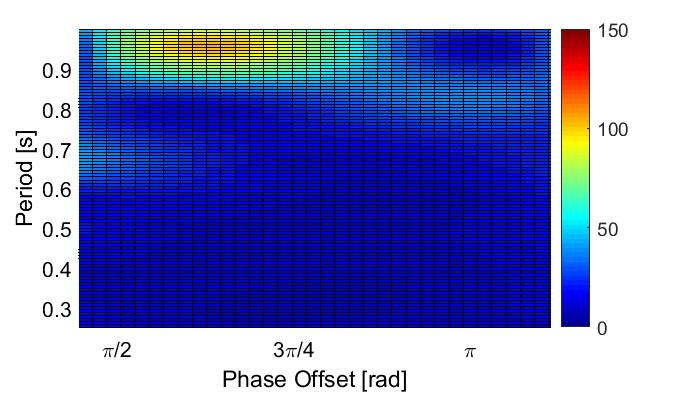
\includegraphics[width=0.53\textwidth]{unsync}
           \caption{CoT for left/right anti-symmetric gaits at smaller periods}
           \label{fig:unsync_gait_2}
\end{figure}
           


\section{Discussion}

% Assigned: Thu/Ash


% Outline:
% Paragraph 1. Identified several independent gait patterns, that agree with quadruped patterns from {Hildebrand701}
%  - List gaits, appropriate patterns, ID location on CoT plots


% Paragraph 2. Future work
%  - Will examine GRFs and ground contact patterns to compare w/ horse paper
%  - Will compare leg angle to passive walking/SLIP models
% That's good enough. Done. No time or space to write much more.
The framework developed has been studied under elliptical pattern with emphasis on the fore lag and period of gait. Given the same path trajectory for all gaits, the optimal gait parameters for left/right symmetry was a 0.58s period with a phase offset of 1.1$\pi$ while left/right anti-symmetry had an optimal gait at a 0.33s period and 0.9$\pi$ offset, corresponding to a bounding and trotting gait, respectively. Frames showing each gait are given in \cref{fig:sym_gait,fig:asym_gait}. In Hildebrand's study, horse footfalls were shown throughout a stride in several types of gaits. In running trots, the phase offset between the fore and rear legs was approximately $\pi$, which is similar to the \emph{Minitaur}'s optimal gait of 0.9 $\pi$ phase offset \autocite{Hildebrand701}. 

\begin{figure}[t!]
    \centering
    \begin{subfigure}[t]{0.45\linewidth}
        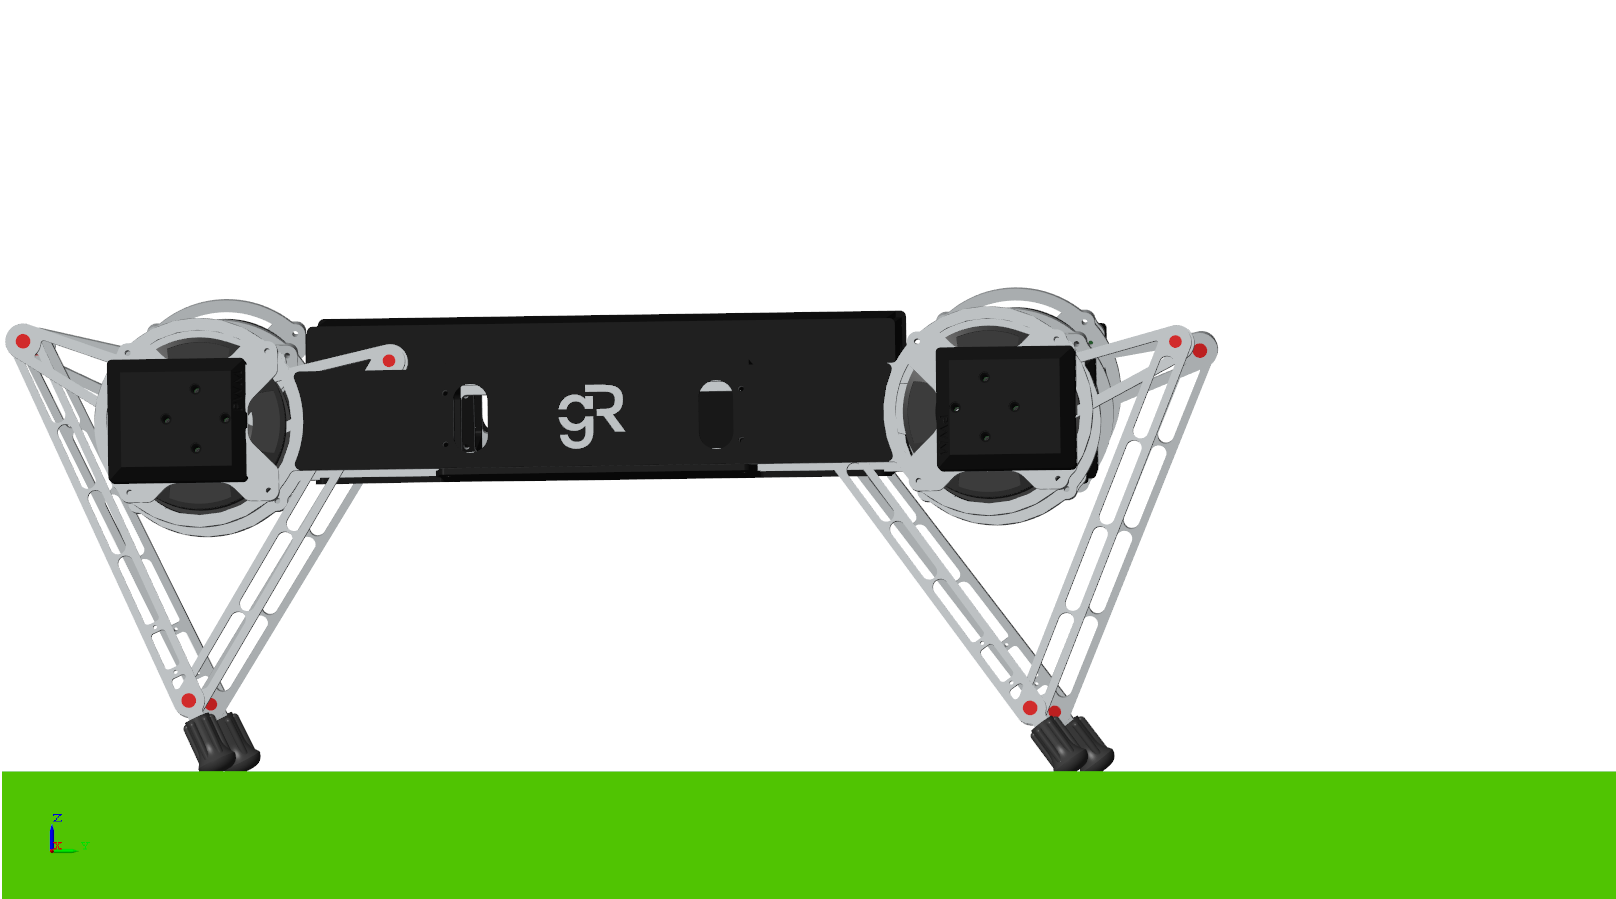
\includegraphics[width=\textwidth]{symm_snap1}
        \caption{State 1}
    \end{subfigure}%
    \begin{subfigure}[t]{0.45\linewidth}
        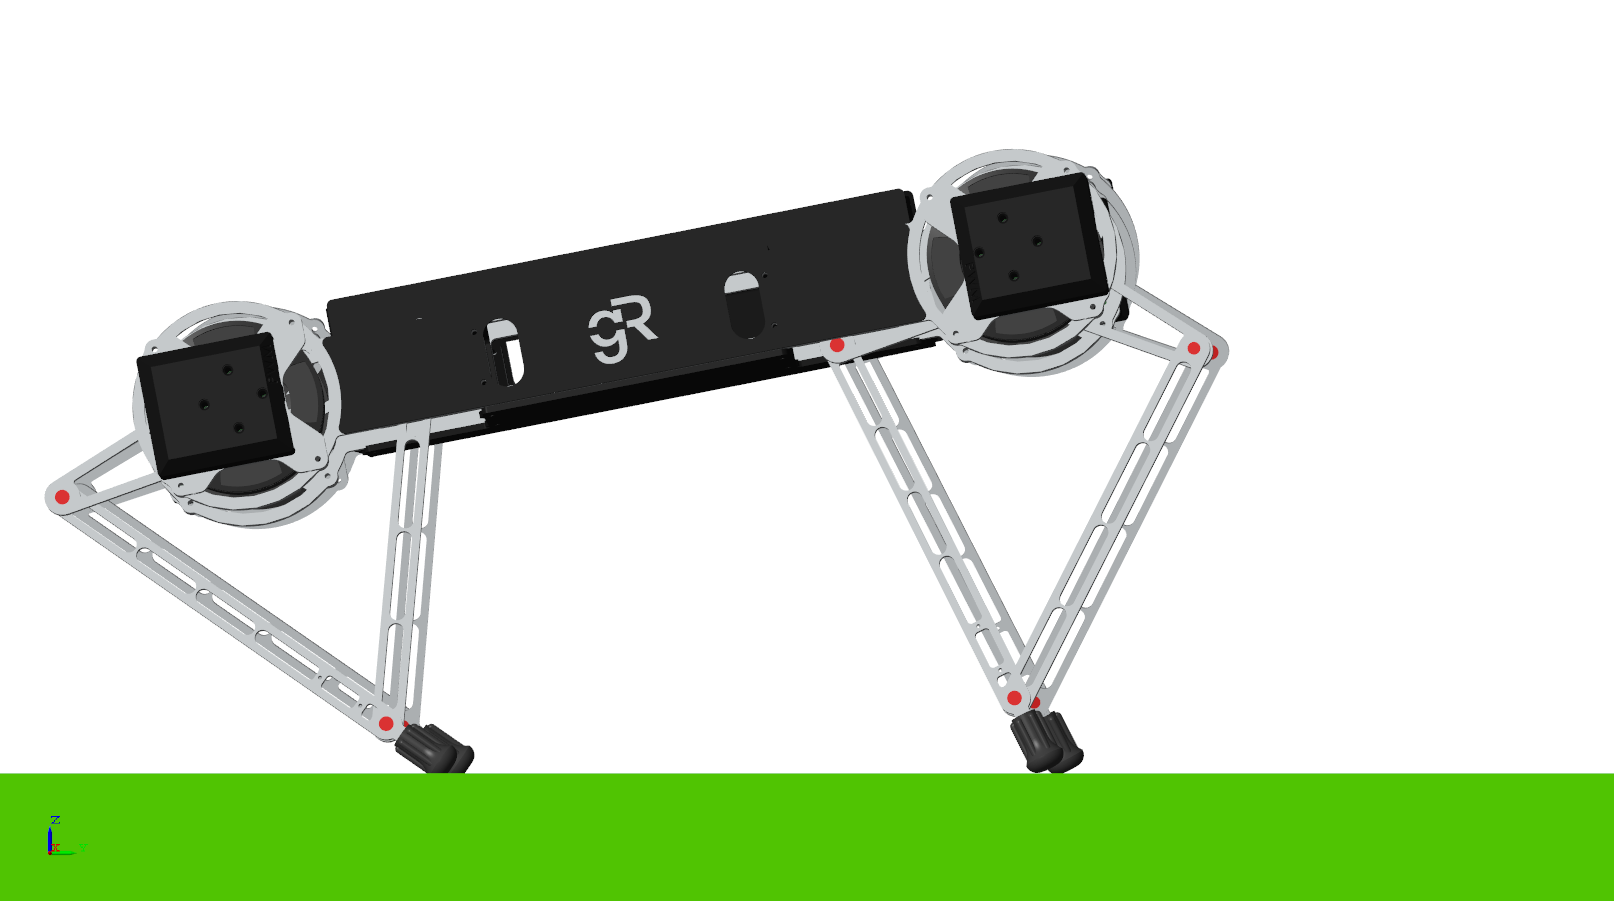
\includegraphics[width=\textwidth]{symm_snap2}
        \caption{State 2}
    \end{subfigure} \\
    \begin{subfigure}[t]{0.45\linewidth}
        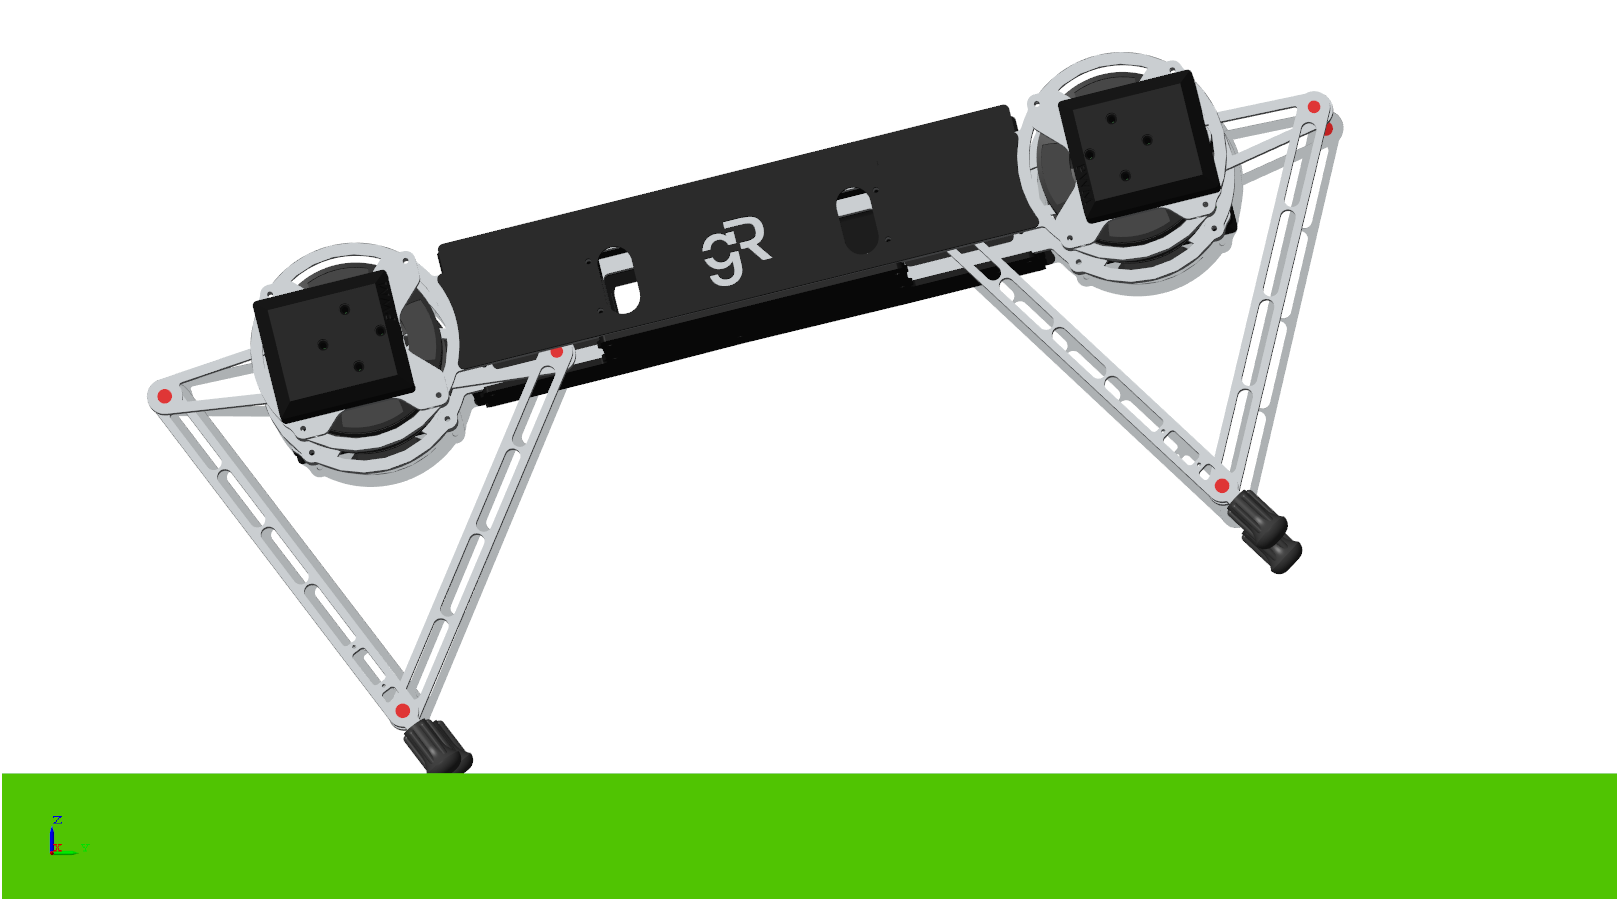
\includegraphics[width=\textwidth]{symm_snap3}
        \caption{State 3}
    \end{subfigure}%
    \begin{subfigure}[t]{0.45\linewidth}
        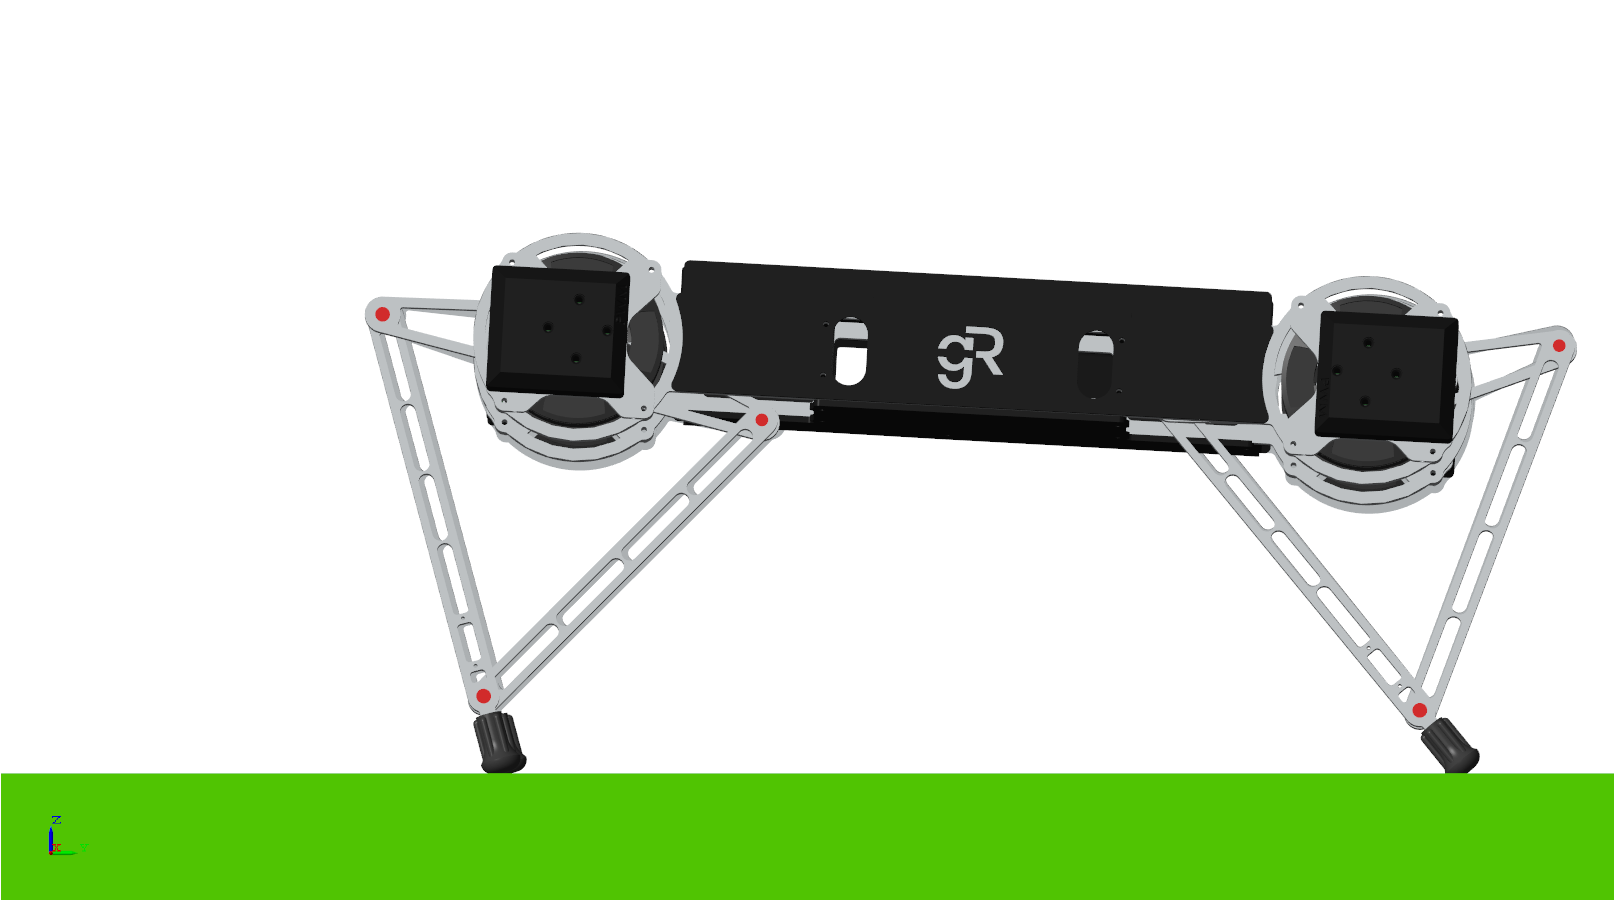
\includegraphics[width=\textwidth]{symm_snap4}
        \caption{State 4}
    \end{subfigure}%
    \caption{Sample symmetric gait with \emph{period} $0.58 s$, \emph{lag} $1.12\pi$.}
    \label{fig:sym_gait}
\end{figure}

\begin{figure}[t!]
    \centering
    \begin{subfigure}[t]{0.45\linewidth}
        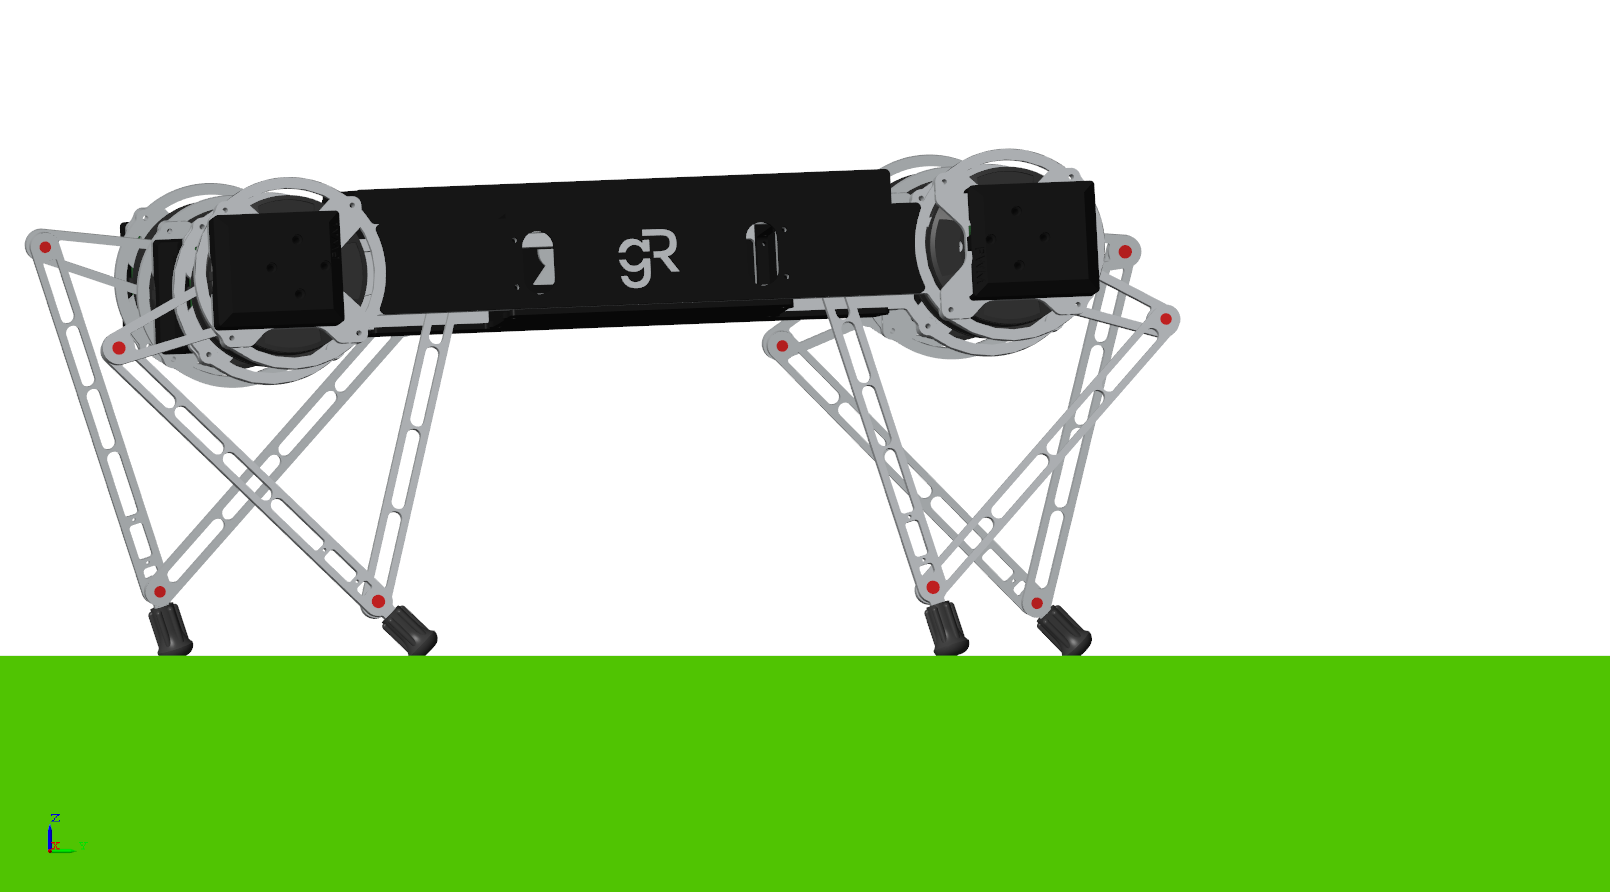
\includegraphics[width=\textwidth]{asymm_snap1}
        \caption{State 1}
    \end{subfigure}%
    \begin{subfigure}[t]{0.45\linewidth}
        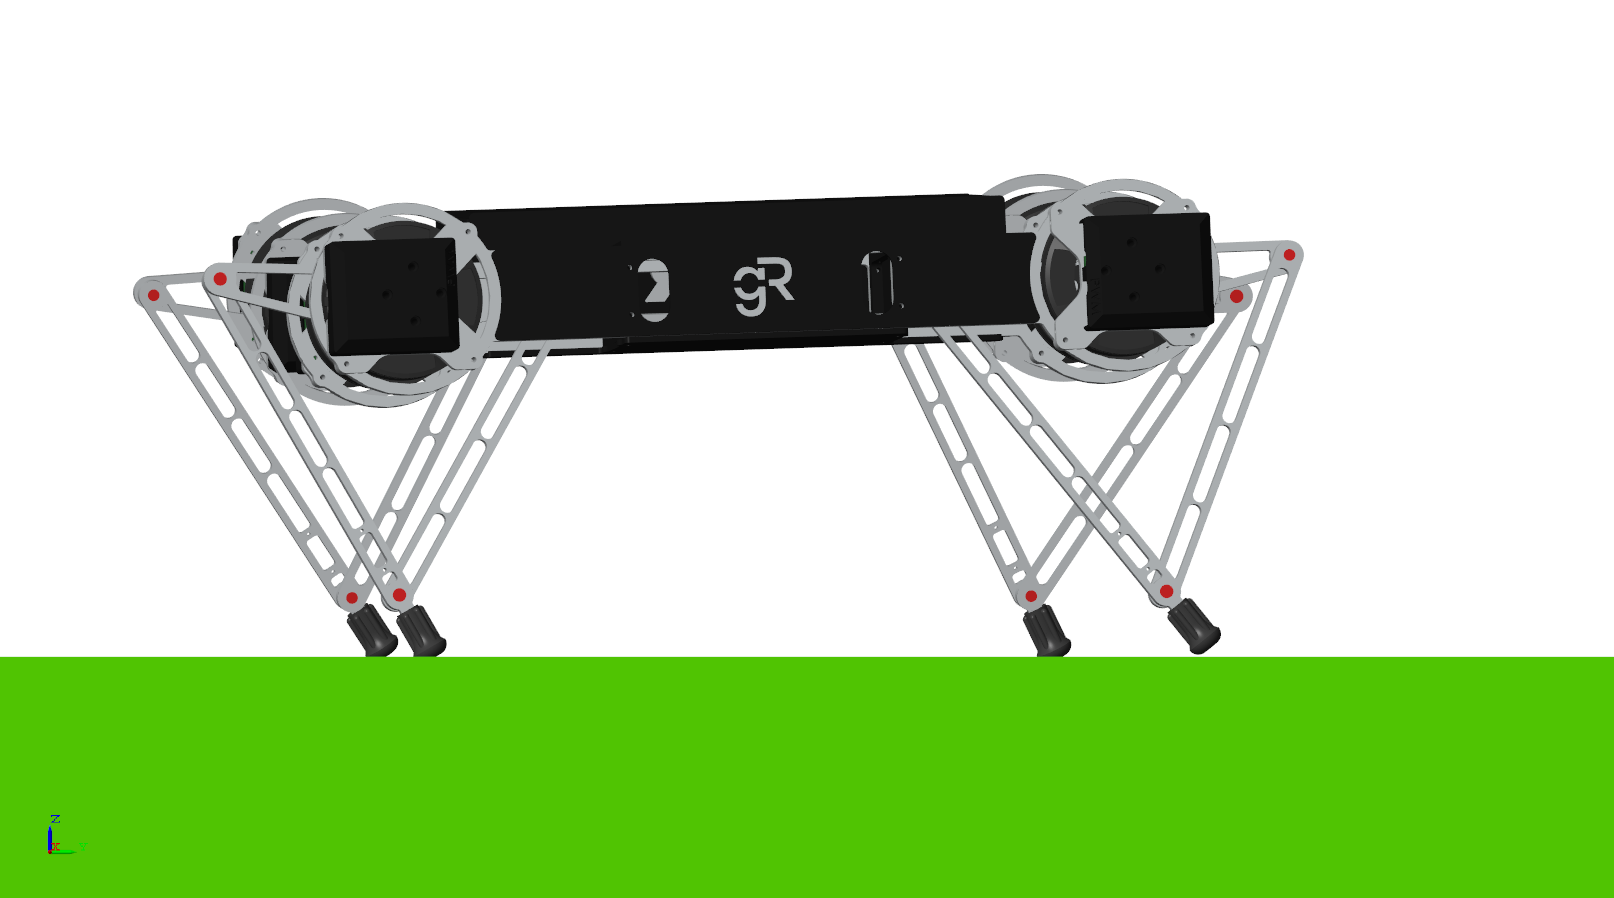
\includegraphics[width=\textwidth]{asymm_snap2}
        \caption{State 2}
    \end{subfigure} \\
    \begin{subfigure}[t]{0.45\linewidth}
        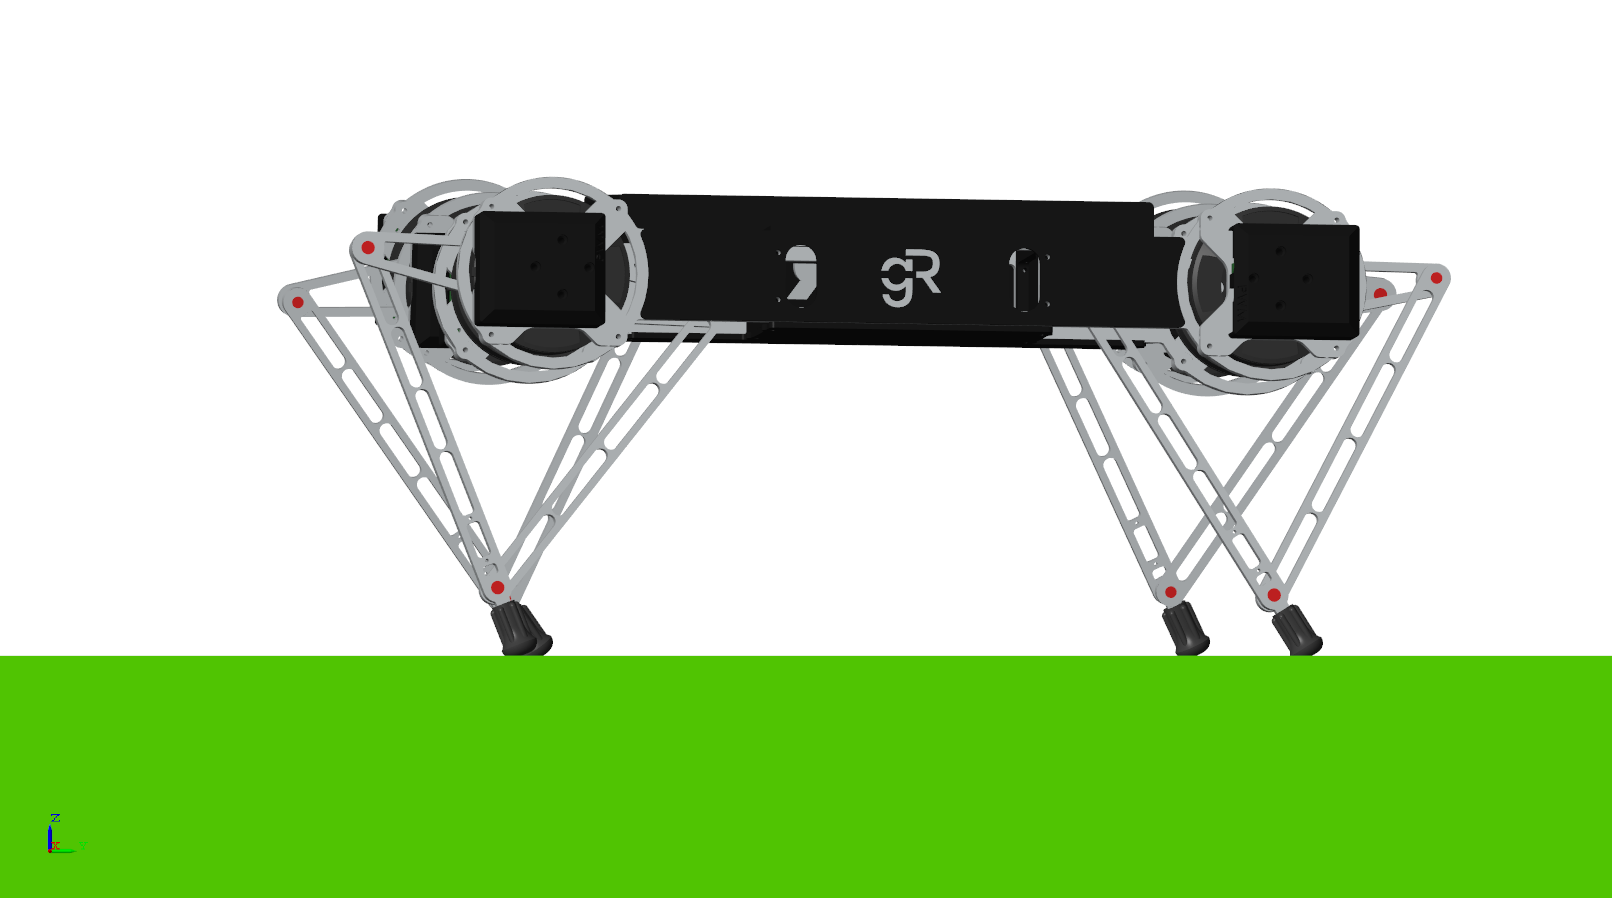
\includegraphics[width=\textwidth]{asymm_snap3}
        \caption{State 3}
    \end{subfigure}%
    \begin{subfigure}[t]{0.45\linewidth}
        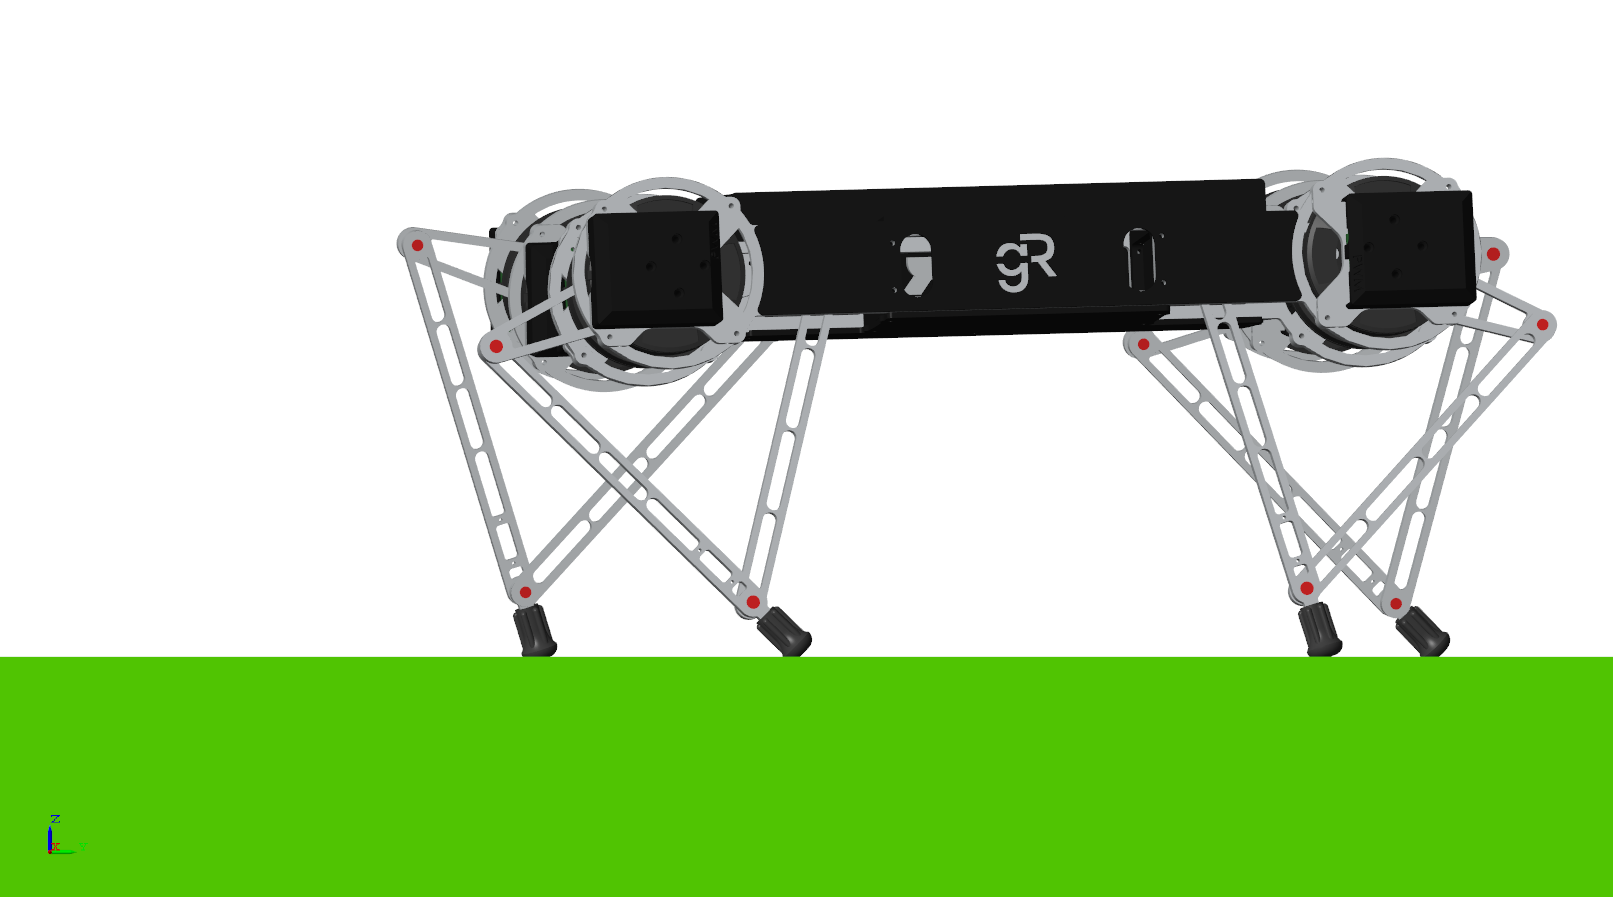
\includegraphics[width=\textwidth]{asymm_snap4}
        \caption{State 4}
    \end{subfigure}%
    \caption{Sample asymmetric gait with \emph{period} $0.33 s$, \emph{lag} $0.9\pi$.}
    \label{fig:asym_gait}
\end{figure}

\subsection{Limitations}
The CoT for our models were much higher than in biological systems. The minimum CoT that we found were 34.6 for left/right symmetric gaits and 11.5 for anti-symmetric gaits while biological systems tend to have CoT values around 0.1-0.15. These inefficiencies from the simulation could have come from poor tuning of the motor controllers. Because we were interested in energy cost due to different gait parameters, we did not optimize the PID gains for the motor controller. Due to the speed of the simulator, we were limited in the number of parameters that we could choose to search. We decided that leg timing was more important than path trajectory for gait generation, so we selected leg timing parameters to optimize. 

\subsection{Future Directions}
Because gaits have different optimal path trajectories, we plan to optimize the elliptical path trajectories at the optimal parameters for period and phase offsets found also using CMA-ES.
We plan to extend the study by developing realistic foot trajectory patterns observed in quadrupeds to achieve results that are in correlation with ground reaction forces observed in quadrupeds. We also plan to use impedance control rather than position control for the motors. Lastly, we want to look into developing more advanced control architectures in order to improve robustness to uncertainty and disturbances in the environment. 


% use section* for acknowledgment
\section*{Acknowledgment}

The author would like to thank Professor Chris Atkeson for overseeing this independent study, as well as Thu Nguyen (formerly a graduate student at CMU, presently at Stanford) for her previous contributions to the project. Additionally, the author would also like to acknowledge Ghost Robotics LLC for supporting this work by providing design files of the \emph{Minitaur} robot platform for this work. 

% references section
\nocite{*}
\printbibliography

% that's all folks
\end{document}


